%%%%%%%%%%%%%%%%%%%%%%%%%%%%%%%%%%%%%%%%%
% Friggeri Resume/CV
% XeLaTeX Template
% Version 1.2 (3/5/15)
%
% This template has been downloaded from:
% http://www.LaTeXTemplates.com
%
% Original author:
% Adrien Friggeri (adrien@friggeri.net)
% https://github.com/afriggeri/CV
%
% License:
% CC BY-NC-SA 3.0 (http://creativecommons.org/licenses/by-nc-sa/3.0/)
%
% Important notes:
% This template needs to be compiled with XeLaTeX and the bibliography, if used,
% needs to be compiled with biber rather than bibtex.
%
%%%%%%%%%%%%%%%%%%%%%%%%%%%%%%%%%%%%%%%%%

\documentclass[]{friggeri-cv} % Add 'print' as an option into the square bracket to remove colors from this template for printing
\usepackage{graphicx}
\graphicspath{ {images/} }

\begin{document}

\header{Stefano}{Munarini}{Software Developer} % Your name and current job title/field

%----------------------------------------------------------------------------------------
%	SIDEBAR SECTION
%----------------------------------------------------------------------------------------

\begin{aside} % In the aside, each new line forces a line break
% 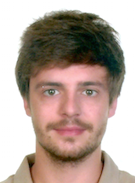
\includegraphics[scale=0.5]{fototessera}
\section{contact}
Jämeräntaival 6 B 207
Otaniemi, Espoo, 02150
+358 (0) 46 9424916
\href{mailto:stefano.munarini@me.com}{stefano.munarini@me.com}
\textbf{Skype}:
stefano.munarini
\section{accounts}
\href{https://it.linkedin.com/in/munarinistefano}{\textbf{LinkedIn}:
munarinistefano}
\href{https://github.com/munarinistefano}{\textbf{GitHub}:
munarinistefano}
\href{http://stackexchange.com/users/2741833/stefano-munarini}{\textbf{StackOverflow}:
2741833}
\section{languages}
Italian mother tongue
English proficient
\section{programming}
Python, Java, SQL, 
HTML, Javascript
\section{certifications}
IELTS Bandscore 7
\end{aside}

%----------------------------------------------------------------------------------------
%	ABOUT ME SECTION
%----------------------------------------------------------------------------------------


\section{about me}
{
	A passionate and well-rounded developer, with an high capacity of problem solving, who is able to convert complex problems into smaller and easier tasks. A good team player but also a team leader if needed, who is able to listen and to compare ideas with others to drive teams to better solutions. \\
	A good background in web development with Python, Django, JavaScript, MySQL, PostgreSQL, Docker, Cron and Git achieved during his work experience in London, starting as an intern in a startup called TutorCruncher and continued as Python Developer at Tangent Snowball, a digital agency responsible for developing projects for clients such as PepsiCo, Sky, Carlsberg, Wolseley and many more. \\
	A good background in Android development confirmed by the popularity (over 90k downloads) and the rating (4.5/5) of his application “Libretto Universitario" in the Google Play Store, and certified by the winning of the first price as “Best mobile application of 2013” at the UpperApp festival. A good academic background in web development with Java technologies, as well as with the Spring framework.
	\\
	A natural explorer and a traveler who had met lots of different cultures that enabled him to open his mind while teaching him values such as respect, adaptability and integrity.
}

%----------------------------------------------------------------------------------------
%	WORK EXPERIENCE SECTION
%----------------------------------------------------------------------------------------

\section{experience}

{Feb 2016 -- Jul 2016} \\
{\textbf{Python Developer}} \\
{\href{http://www.tangentsnowball.com}{Tangent Snowball}} -- {London, UK} \\
{This role encompassed the development of CRM platforms for companies such as PepsiCo and Walkers. In particular, I was responsible for the development of a eCRM web platform for Wolseley and for the development and the maintenance of the Counts For More platform (PepsiCo). \\
The technology stack was made of Python (Django), JavaScript, HTML, MySQL, PostgreSQL, Docker, Git and Jira.}

% \subsection{Internship}

{Jan 2016 -- Feb 2016} \\
{\textbf{Python Developer}} \\
{\href{http://www.tutorcruncher.com}{TutorCruncher}} -- {London, UK} \\
{Responsible for developing, improving and extending functionalities of TutorCruncher, a cloud-based platform developed in Django.}

{Feb 2014 -- Jun 2014} \\
{\textbf{Android Developer}} \\
{\href{http://www.dedagroup.it}{Dedagroup ICT Network}} -- {Trento, Italy} \\
{Responsible for designing and developing an Android application aimed at helping people affected by Alzheimer's Disease. The role encompassed all aspects of software design, both fronted and backend, including architectural decisions.}

%----------------------------------------------------------------------------------------

%\subsection{Part Time}


%----------------------------------------------------------------------------------------
%	PROJECT SECTION
%----------------------------------------------------------------------------------------

\section{projects}

{Jul 2013 -- Sep 2015} \\
{\href{https://play.google.com/store/apps/details?id=com.povodev.libretto}{\textbf{Libretto Universitario}}} \\
{https://play.google.com/store/apps/details?id=com.povodev.libretto} \\
{Libretto Universitario is an Android application for Italian university students, which aims at helping and simplifying the management and the organization of one's university career. It is available for the download in the italian Google Play Store.}
% \\
%------------------------------------------------

% {Feb 2014 -- May 2014} \\
% {\href{https://github.com/stestisa/Hemme_Backend}{\textbf{HEMME}}} \\
% {HEMME is a mobile application developed during the internship, which was committed by a customer and which aims at helping people affected by Alzheimer's Disease, their tutors and their doctors.
% I was responsible for the communication with the customer, the design and the development of both the backend and the mobile application.}
% \\
%------------------------------------------------

% {Oct 2013 -- Dec 2013} \\
% {\href{https://github.com/stestisa/StudentsChat}{\textbf{Student's Chat}}} \\
% {University project (\textit{Web Programming} course, marked 28/30)} \\
% {Student's chat is a web application developed with Java technologies (Servlet, JSP, Filter). I was responsible for the design and the development of this application, as well as the configuration and the design of the database.}
% \\
% %------------------------------------------------

% {Feb 2012 -- May 2012} \\
% {\href{https://github.com/stestisa/aMuse_Backend}{\textbf{aMuse}}} \\
% {University project (\textit{Software Engineering} course, marked 30/30)} \\
% % {Youtube video: RAYp5kO0W4} \\
% {aMuse is both a web and a mobile application (for the Android platform), which was developed as a University project with 5 other classmates, which aims at enhancing one's museum visit. While the mobile application allows to scan QR codes, get information about the artworks scanned and create personal books, the web application allows to browse and share them with family and friends. \\
% I was responsible for the development of the mobile application and I also led the mobile team I was working with.}

%----------------------------------------------------------------------------------------
%	AWARDS SECTION
%----------------------------------------------------------------------------------------

\section{awards}

{Dec 2013} \\
{\textbf{\href{http://www.upperapp.it}{UpperApp Festival} - 1\textsuperscript{st} Prize: Best Mobile Application of 2013} \\
{Agorà Telematica} \\
Libretto Universitario has been awarded as \textit{Best Mobile Application} of 2013 at the UpperApp Festival.}
 % 1\textsuperscript{st} Edition.}

%----------------------------------------------------------------------------------------
%	EDUCATION SECTION
%----------------------------------------------------------------------------------------

\section{education}

%\begin{entrylist}

%\entry
{2016 -- 2017} \\
\textbf{EIT Digital Master School} \\
\textbf{Master Degree {\normalfont in Information Networks}} \\
{Aalto University, Finland (Entry University)} \\
{Major: Software and Service Architectures (SSA) \\
Minor: Innovation \& Entrepreneurship (I\&E)}

{2011 -- 2015} \\
\textbf{Bachelor Degree {\normalfont in Computer Science}} \\
{University of Trento, Italy}


%----------------------------------------------------------------------------------------
%	CERTIFICATE SECTION
%----------------------------------------------------------------------------------------

% \section{certifications}

% {Dec 2015} \\
% {\textbf{IELTS} Bandscore 7 %(Listening , Reading, Writing, Speaking)}

% {Apr 2015} \\
% {\href{https://certs.duolingo.com/ud85gf8c}{\textbf{Duolingo Proficiency Exam} in English: Proficient}}

% {2010} \\
% {\textbf{ECDL}: European Computer Driving Licence}

% {2008} \\
% {\textbf{Trinity GESE}: B2 of the CEFR}

%----------------------------------------------------------------------------------------
%	INTERESTS SECTION
%----------------------------------------------------------------------------------------

% \section{interests}

% \textbf{professional:} software design, web and mobile applications development, programming
% \textbf{personal:} travel, photography, vinyls, running, hiking

\end{document}